\documentclass[12pt]{article}

\usepackage{colortbl}
\usepackage{amsmath}
\usepackage{amssymb}
\usepackage{appendix}
\usepackage{subfigure}
\usepackage{empheq}
\usepackage{framed}
\usepackage[USenglish]{babel}
\usepackage{graphicx}
\usepackage[margin=1.0in]{geometry}
\setcounter{tocdepth}{3}

\usepackage{pdfpages}

\usepackage{eurosym}
\usepackage{mathpazo} 
\usepackage{booktabs}

\def\betabold{{\pmb{$\beta$}}}

%
\begin{document}

\date{November 6, 2019}

\title{
\centerline{}
\centerline{}
\centerline{}
ETEAPOT EDM Benchmark I: Updated Results:
}
\author{J. D. Talman and R. M. Talman
}

\maketitle

% \tableofcontents

\begin{abstract}
This chapter repeats and updates benchmark lattice investigations first performed 
using the ``all-electric'' code ETEAPOT in 2012 for all-electric proton EDM rings. 
The lattice electric bending fields for the three files have indices $m=-1$, 
$m\approx0$, and $m=1$. Values of horizontal and vertical tunes, and beta 
functions at the origin (midway between adjacent bends) are tabulated. 
Results are compared to values obtained from a linearized transfer matrix 
formalism. In all cases the design vertical tunes have been adjusted to 
$Q_y$=0.2.
\end{abstract}
%

\clearpage

\section{Introduction}
All-electric lattices for a storage ring to measure the electric
dipole moment (EDM) of the proton are described in a CERN Yellow Report,
CERN-2019-001-M, ``Feasibility Study for a Storage Ring to Search for EDMs
of Charged Particles''. Earlier designs were contained in a BNL
proposal by the Storage Ring EDM Collaboration, \emph{A Proposal to Measure the
Proton Electric Dipole Moment with $10^{-29}\,$e-cm Sensitivity}\cite{pEDM}.
The lattices studied here have been stripped down to their bare essentials
in order to simplify benchmark comparisons of various simulation
codes. All results using ETEAPOT in an (unpublished) 2012 benchmark report
(to the DOE, in connection with their financial support at the time) 
are replicated using (updated) ETEAPOT in the present report. 

An electric field with index $m$ power law dependence on radius $r$,
for $y$=0, is
%
\begin{equation}
{\bf E}(r,0)
 = 
-E_0\,\frac{r_0^{1+ m }}{r^{1+ m }}\,{\bf\hat r},
\label{eq:WeakFoc.1m}
\end{equation}
%
and the electric potential $V(r)$, adjusted to vanish (on the storage ring 
design orbit) at $r=r_0$, is 
%
\begin{equation}
V(r)
 =
-\frac{E_0r_0}{ m }\,
\bigg(
\frac{r_0^m }{r^m }
 -
1
\bigg).
\label{eq:WeakFoc.2m}
\end{equation}
%
The ``cleanest'' case theoretically has $m$=1, in which case it is known
as the Kepler or the Coulomb electric field. Our problem is a
bit more general than this non-reletivistic terminology suggests, since our
treatment is necessarily relativistic. For $m$=1 the
Kepler problem can be solved with the same generality
in the relativistic as in the nonrelativistic case; but the
orbits are no longer exactly elliptical, nor exactly closed
however\cite{Munoz}.

The full rings simulated in this chapter are circular and consist of 40 identical cells. 
A single cell is shown in Figure~\ref{fig:E_benchmark}. With curved planar plates (which is 
the easiest configuration to construct) the electrodes are
concentric cylinders and the field index is $m$=0. The 
optimal (i.e. longest) spin coherence time (SCT) is expected to be close 
to this zero m-value. (For $m$=1 the electrodes would be concentric spheres.)

For $m$=0 the fields are independent of vertical displacement $y$,
which implies that there is no vertical focusing provided by the bending field.
Provision of vertical stability therefore requires 
focusing quadrupoles; they are labeled $q$ in Figure~\ref{fig:E_benchmark}.
Even if not required for vertical stability, the $q$ quadrupoles are 
necessary for adjusting the vertical tune $Q_y$ of the storage ring.
The vertical tunes have been adjusted to $Q_y=0.2$ for all three of
the benchmark lattices described in the following sections.

\section{Parameters of Benchmark Lattices}
%
\begin{figure}[h]
\centering
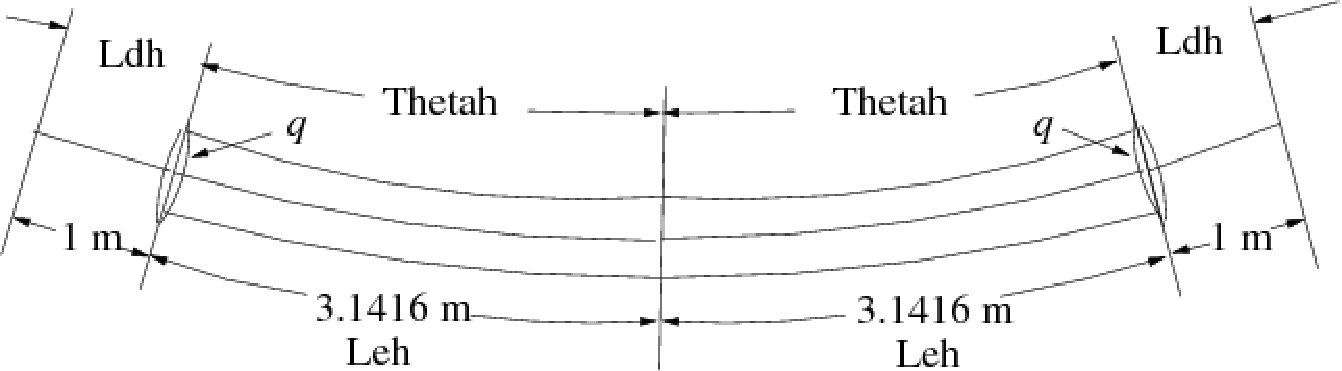
\includegraphics[scale=0.5]{pdf/E_benchmark-latt.pdf}
\caption{\label{fig:E_benchmark}Single cell geometry. The full lattice consists
of 40 identical cells.}
\end{figure}
%

Analytic, linearized transfer matrix MAPLE programs with names {\tt E\_BM\_P1.0.mw}, 
{\tt E\_BM\_Z.mw}, and {\tt E\_BM\_M1.0.mw}
are in {\tt /home/talman/EDM/EDM-lattice/maple/benchmark} directory. The corresponding SXF 
lattice files are produced in {\tt /home/oxygen/XML2ADXF} and {\tt /home/oxygen/ADXF2SXF/}.
The filenames are column headings in the following table, which contains lattice parameters,
as calculated by MAPLE.
%
\begin{table}[h]
\caption{\label{tbl:benchmarkParams}Parameters of benchmark all-electric EDM lattices, 
and Twiss parameters calculated from linearized transfer matrices. Note that the 
``half bend'', and ``half drift'' elements are treated as individual elements in 
the sxf file. This gives 80 bends. The software treats these as 160 bends after slicing.
} 
\medskip
\centering
\begin{tabular}{|c|c|c|c|c|c|c|c|c|}           \hline
file name         & variable name     & unit & {\tt E\_BM\_M1.0.sxf} & {\tt E\_BM\_Z.sxf} & {\tt E\_BM\_P1.0.sxf} \\ \hline
cells/arc         & {\tt NCellPerArc} &      &      20               &       20           &        20             \\
bend radius       &  {\tt r0}         &  m   &     40.0              &      40.0          &       40.0            \\
half drift length &  {\tt Ldh}        &  m   &      1.0              &     1.0            &        1.0            \\
half bend per cell & {\tt Thetah}     &  r   &   0.078539816         &  0.078539816       &  0.078539816          \\
half bend length  & {\tt Leh}         &  m   &    3.141592           &  3.141592          &   3.141592            \\
circumference     & {\tt circum}      &  m   &   331.327             &   331.327          &    331.327            \\ \hline
inverse focal length &  {\tt q}       & 1/m  &    -0.002019          & -0.00005960        &     0.0019075         \\
field index       &  {\tt m}          &      &     -1.0              &  1.0e-10           &         1.0            \\ \hline
horizontal beta  & {\tt betax}       &  m   &    35.9237            &  36.1018           &     36.1910            \\
vertical beta     & {\tt betay}       &  m   &   264.182             &  263.620           &     262.237            \\ \hline
horizontal tune  &  {\tt Qx}         &      &     1.4605            &   1.4578           &      1.4588            \\
vertical tune     &  {\tt Qy}         &      &     0.20024           &   0.20004          &     0.20047            \\
\hline
\end{tabular}
\end{table}
%

\section{Twiss Parameter Extraction}
A once-around (``monodromy'' in mathematical terminology) 
transfer matrix at any point in the ring has the standard Twiss parameterization,
%
\begin{equation}
 \bf{M} =
  \begin{pmatrix}
           \cos\mu + \alpha \sin\mu &            \beta \sin\mu \\
   -\frac{1+\alpha^2}{\beta}\sin\mu & \cos\mu - \alpha \sin\mu
  \end{pmatrix}.
\label{eq:Twiss.1}
\end{equation}
%
At a mirror symmetry point in the lattice, as here, though not in general, $\alpha$ vanishes.
The phase advance $\mu$ = 2$\pi Q$ can be obtained from
\begin{equation}
 \cos\mu=\frac{M_{11}+M_{22}}{2}, \quad \hbox{and} \quad M_{12}=\beta \sin\mu.
\label{eq:Twiss.2}
\end{equation}
This has assumed that $\beta$ is, by definition, positive.
These equations determine the signs of both $\cos\mu$ and $\sin\mu$. Reading counter-clockwise, the four 
consecutive phase space quadrants, I/II/III/IV, are characterized by cosine, sine sign pairs 
++/-+/- -/+-, respectively. We then obtain the fractional parts of the phase advance from 
%
\begin{equation}
 \mu = 
\begin{cases} 
       \cos^{-1}( \frac{M_{11}+M_{22}}{2} ), & \mbox{if } \textnormal{quadrant}\mbox{ is I or II} \\ 
  2\pi-\cos^{-1}( \frac{M_{11}+M_{22}}{2} ), & \mbox{if } \textnormal{quadrant}\mbox{ is III or IV} \end{cases}.
\label{eq:Twiss.3}
\end{equation}
%
This still only partially resolves the aliasing ambiguity. Resolving the integer tune ambiguity requires 
keeping track of phase space quadrants while tracking through the lattice. To avoid error in this
process it is important for sampling intervals small enough that no phase quadrant can be skipped.
This keeping track of the integer tune is indicated in captions 
to graphs below. We then obtain $\beta$ from Eq.~(\ref{eq:Twiss.2}), and $\alpha$ from 
%
\begin{equation}
 \alpha=\frac{M_{11}-M_{22}}{2\sin\mu}.
\label{eq:Twiss.4}
\end{equation}
%
It is because the TEAPOT family of codes use only particle tracking, and no transfer matrices in
studying ring behavior---transfer matrix components, and Twiss and other lattice functions are only 
obtained for the purpose of comparing results with more conventional accelerator simulation codes.

\section{ETEAPOT tune determinations and analytic comparisons}
\subsection{Data collection organization}
In all cases, $m=1,0,-1$, the lumped Q-quadrupoles strengths, $q$, were adjusted to produce vertical
tune $Q_y=0.2$. Values of $q$ are given in the graph titles.
For each of the three benchmark lattices, bunches of 21 standard particles are 
tracked for one turn. Each of the 80 bend elements is sliced in half for this (and all other) analyses. 
The graphs show horizontal and vertical displacements for two of the standard particles at the exits from 
each of the bends. Both transverse tune determinations are shown in the figure captions. 

Once-around transfer matrices are obtained from the 21 standard particles using numerical differences. 
This differencing is based on the smallness (typically 1\,$\mu$m spatial displacement, 1\,$\mu$r 
angular displacement) of the initial offsets. Sensitivity to this choice is investigated in 
Table~\ref{tbl:benchmarkParams.P1.0} and other tables. Twiss parameters, $\beta_x, \beta_y$, and 
$\mu_x, \mu_y$ are calculated using the procedures already described. The fractional and integer tunes 
are obtained from the graphs the following the tables.

Dependence of the lattice parameters on ``differencing'' displacement {\tt tiny} are shown in 
Tables~\ref{tbl:benchmarkParams.P1.0}, \ref{tbl:benchmarkParams.Z}, and \ref{tbl:benchmarkParams.M1.0}.

Each bend element in any SXF lattice description file corresponds to a single bend element in
an actual ring and is therefore referred to as a ``single bend''. By the internal construction of ETEAPOT, 
each such bend is sliced at least once, or (optionally) more times. 

Because the ``cylindrical'' $m=0$ electrode shape choice is considered to be the most favorable,
more dependencies are investigated for $m=0$ than for $m=\pm1$. In particular the effect of 
``artificial pre-slicing'' is investigated for $m=0$.

\clearpage

\subsection{Lattice E\_BM\_P1.0, $m=1$, ``spherical'' bending results}
\subsubsection{Two ETEAPOT slices per bend}
Table~\ref{tbl:benchmarkParams.P1.0} shows the lattice parameters obtained
with $m=1$, ``spherical'' bending, with minimal ETEAPOT slicing of 2 slices per bend.
ETEAPOT results agree well with analytic lattice calculations using MAPLE. The 
accuracy of ``differentiation by differencing'' is investigated. The effect of
increasing the unit differencing value ${\tt tiny}=10^{-6}$ by two orders of manitude
has negligible effect on the lattice parameters, showing that the differencing provides
sufficient accuracy.

\begin{table}[h]
\caption{\label{tbl:benchmarkParams.P1.0}E\_TEAPOT comparisons for
{\tt ./tracker ./data/E\_BM\_P1.0.sxf 30 1 > \& ! JTout}.
All {\tt typ} numerical differentiation displacements are proportional to {\tt tiny}.} 
\medskip
\centering
\begin{tabular}{|c|c|c|c|c|c|c|c|c|}           \hline
file name         & variable name     & unit  &   linearized  & 2 slices/bend & $\Delta$'s  \\ 
                  &                   &       &   MAPLE       &  ETEAPOT      &             \\ \hline
cells/arc         & {\tt NCellPerArc} &       &        20     &               &             \\
bend radius       &  {\tt r0}         &  m    &       40.0    &               &             \\
half drift length &  {\tt Ldh}        &  m    &        1.0    &               &        \\
half bend per cell & {\tt Thetah}     &  r    &  0.078539816  &               &        \\
half bend length  & {\tt Leh}         &  m    &   3.141592    &               &        \\
circumference     & {\tt circum}      &  m    &    331.327    &               &        \\ 
inverse focal length &  {\tt q}       & 1/m   &     0.0019075 &               &        \\
field index       &  {\tt m}          &       &         1.0   &               &         \\ \hline 
{\tt tiny=1.0e-6} &                   &       &               &               &          \\ \hline
horizontal beta   & {\tt betax}       &  m    &      36.1910  &  36.1910      & 0.0000        \\
vertical beta     & {\tt betay}       &  m    &    262.2370   &  262.2370     & 0.0000        \\
horizontal tune   &  {\tt Qx}         &       &      1.4588   &  1.4588       & 0.0000        \\ 
vertical tune     &  {\tt Qy}         &       &     0.2005    &  0.2005       & 0.0000        \\ \hline
{\tt tiny=1.0e-5} &                   &       &               &               &          \\ \hline
horizontal beta   & {\tt betax}       &  m    &     36.1910   &  36.1910      & 0.0000  \\
vertical beta     & {\tt betay}       &  m    &    262.2370   &  262.2370     & 0.0000  \\ 
horizontal tune   &  {\tt Qx}         &       &      1.4588   &   1.4588      & 0.0000  \\ 
vertical tune     &  {\tt Qy}         &       &     0.2005    &   0.2005      & 0.0000  \\ \hline  
{\tt tiny=1.0e-4} &                   &       &               &               &          \\ \hline
horizontal beta   & {\tt betax}       &  m    &     36.1910   &  36.1925      &  0.0015  \\
vertical beta     & {\tt betay}       &  m    &   262.2370    &  262.2336     & -0.0034       \\
horizontal tune   &  {\tt Qx}         &       &      1.4588   &    1.4588     &  0.0000       \\ 
vertical tune     &  {\tt Qy}         &       &     0.2005    &    0.2005     &  0.0000  \\ \hline
{\tt tiny=1.0e-3} &                   &       &               &               &          \\ \hline
horizontal beta   & {\tt betax}       &  m    &      36.1910  &  36.3349      &  0.1439  \\
vertical beta     & {\tt betay}       &  m    &    262.2370   &  261.8966     & -0.3404 \\
horizontal tune   &  {\tt Qx}         &       &      1.4588   &  1.4589       &  0.0001 \\ 
vertical tune     &  {\tt Qy}         &       &     0.2005    &  0.2006       &  0.0001  \\ \hline
\end{tabular}
\end{table}
%

\begin{figure}[htbp]
  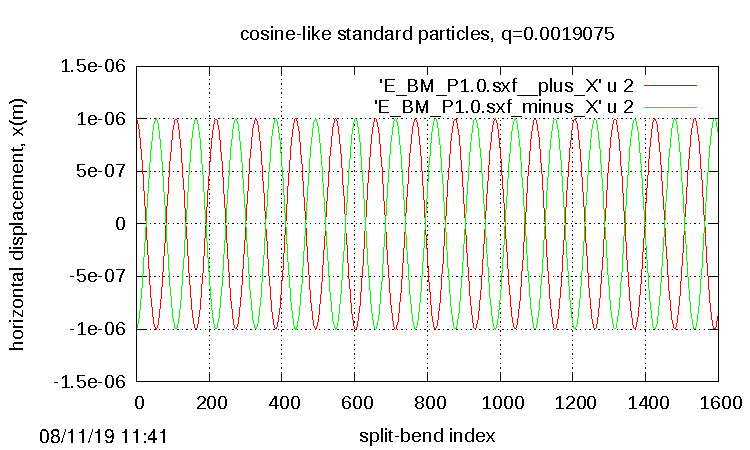
\includegraphics[scale=1.0]{pdf/Fig_I-2t.pdf}
  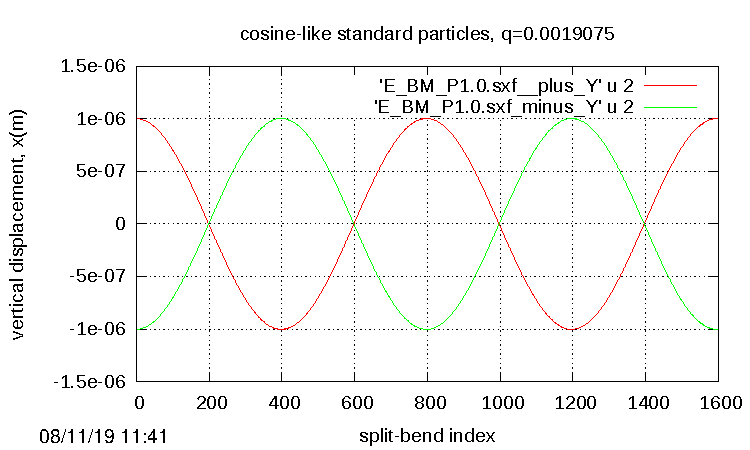
\includegraphics[scale=1.0]{pdf/Fig_I-2b.pdf} 
\caption{Lattice {\tt E\_BM\_P1.0.sxf}; Upper: Horizontal Displacement: 10 turns, 1 sample per split bend. 
$Q_x\approx$ 14.5 osc/10turns=1.45 osc/turn. The integer part of the tune is [$Q_x$] = 1. 
Lower: Vertical Displacement: 10 turns, 1 sample per split bend. $Q_y\approx$ 
2.0 osc/10turns=0.20 osc/turn. The integer part of the tune is [$Q_y$] = 0.}
\end{figure}

\clearpage

\subsection{Lattice E\_BM\_Z, $m=0$, ``cylindrical'' bending results}
\subsubsection{Two TEAPOT slices per bend}
Table~\ref{tbl:benchmarkParams.Z} shows the lattice parameters obtained
with $m=0$, ``cylindrical'' bending, with minimal ETEAPOT slicing of 2 slices 
per bend. Differences between MAPLE theory and ETEAPOT are shown in the final column
of Table~\ref{tbl:benchmarkParams.Z}, though quite small, are not nearly as small
as those obtained in Table~\ref{tbl:benchmarkParams.P1.0}. What makes this 
``not-very-surprising'' is the fact that ETEAPOT evaluates all lattice parameters 
as ``perturbations'' caused by $m$-value deviation away from $m=1$---this deviation 
vanishes for the results in Table~\ref{tbl:benchmarkParams.Z}. By comparing values 
in these two tables the relative importance of differencing and first order 
perturbation can be estimated.

%
\begin{table}[h]\small
\caption{\label{tbl:benchmarkParams.Z}E\_TEAPOTComparisons for
{\tt ./tracker ./data/E\_BM\_Z.sxf 30 0 > \& ! JTout}.
All {\tt typ} numerical differentiation displacements are proportional to {\tt tiny}.
}
\medskip
\centering
\begin{tabular}{|c|c|c|c|c|c|c|c|c|}           \hline
file name         & variable name     & unit  &  linearized  & 2 slices/bend  & $\Delta$'s \\
                  &                   &       &    MAPLE     &  ETEAPOT       &            \\ \hline
cells/arc         & {\tt NCellPerArc} &       &       20     &                &     \\
bend radius       &  {\tt r0}         &  m    &      40.0    &                &     \\
half drift length &  {\tt Ldh}        &  m    &     1.0      &                &     \\
half bend per cell & {\tt Thetah}     &  r    &  0.078539816 &                &     \\
half bend length  & {\tt Leh}         &  m    &  3.141592    &                &     \\
circumference     & {\tt circum}      &  m    &   331.327    &                &     \\ 
inverse focal length &  {\tt q}       & 1/m   & -0.00005960  &                &     \\
field index       &  {\tt m}          &       &  1.0e-10     &                &     \\ \hline
  {\tt tiny=1.0e-6} &                 &       &              &                &     \\ \hline 
horizontal beta  & {\tt betax}       &  m    &  36.1018      &   36.0795      & -0.0223     \\ 
vertical beta     & {\tt betay}       &  m    &  263.6200    &  261.4688      & -2.1512 \\
horizontal tune  &  {\tt Qx}         &       &   1.4578      &    1.4581      &  0.0003 \\
vertical tune     &  {\tt Qy}         &       &   0.2000     &    0.2018      &  0.0018 \\ \hline           
  {\tt tiny=1.0e-5} &                 &       &              &                &      \\ \hline 
horizontal beta  & {\tt betax}       &  m    &  36.1018      &    36.0795     &  -0.0223 \\ 
vertical beta     & {\tt betay}       &  m    &  263.6200    &   261.4688     & -2.1512 \\
horizontal tune  &  {\tt Qx}         &       &   1.4578      &     1.4581     &  0.0003 \\
vertical tune     &  {\tt Qy}         &       &   0.2000     &     0.2018     &  0.0018 \\ \hline           
 {\tt tiny=1.0e-4} &                  &       &              &                &     \\ \hline 
horizontal beta  & {\tt betax}       &  m    &  36.1018      &    36.0809     & -0.0209  \\ 
vertical beta     & {\tt betay}       &  m    &  263.6200    &   261.4654     & -2.1546 \\ 
horizontal tune  &  {\tt Qx}         &       &   1.4578      &     1.4581     &  0.0003 \\
vertical tune     &  {\tt Qy}         &       &   0.2000     &     0.2018     &  0.0018 \\ \hline           
 {\tt tiny=1.0e-3} &                  &       &              &   &     \\ \hline 
horizontal beta  & {\tt betax}       &  m    &  36.1018      &    36.2190     &   0.1172 \\ 
vertical beta     & {\tt betay}       &  m    &  263.6200    &   261.1318     &  -2.4882 \\ 
horizontal tune  &  {\tt Qx}         &       &   1.4578      &    1.4582      &    0.0004 \\
vertical tune     &  {\tt Qy}         &       &   0.2000     &    0.2019      &    0.0019 \\ \hline
\end{tabular}
\end{table}
%

\begin{figure}[htbp]
  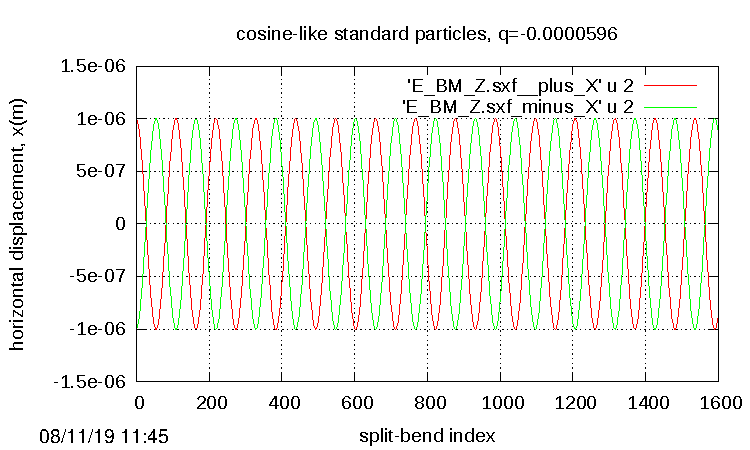
\includegraphics[scale=1.0]{pdf/Fig_I-3t.pdf} 
  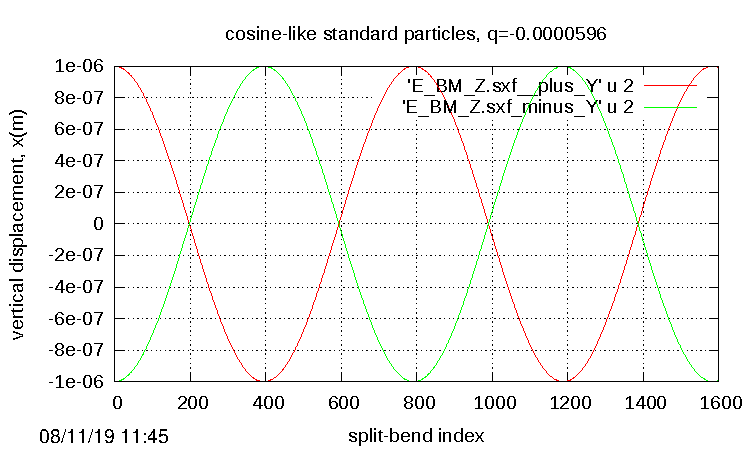
\includegraphics[scale=1.0]{pdf/Fig_I-3b.pdf} 
\caption{Lattice E\_BM\_Z.sxf: Upper: Horizontal Displacement: 10 turns, 1 sample per bend. 
$Q_x\approx$ 14.5 osc/10turns=1.45 osc/turn. The integer part of the tune is [$Q_x$] = 1. 
Lower: Vertical Displacement: 10 turns, 1 sample per bend. 
$Q_y\approx$ 2.0 osc/10turns=0.20 osc/turn. The integer part of the tune is [$Q_y$] = 0.}
\end{figure}

\clearpage
\subsubsection{Ten SXF slices per bend, each with two TEAPOT slices\label{sect:pre-sliced}}
This section investigates the properties of a ``pre-sliced'' SXF lattice
{\tt E-BM-Z-sl.sxf}, which is the same as lattice {\tt E-BM-Z.sxf} except for having
all bends pre-sliced into ten slices. Though there is little horizontal effect,
Figure~\ref{fig:unchanged-q-value} shows that the pre-slicing has actually caused the 
lattice to be vertically unstable. This reflects the extremely weak vertical focusing.

\begin{figure}[htbp] 
  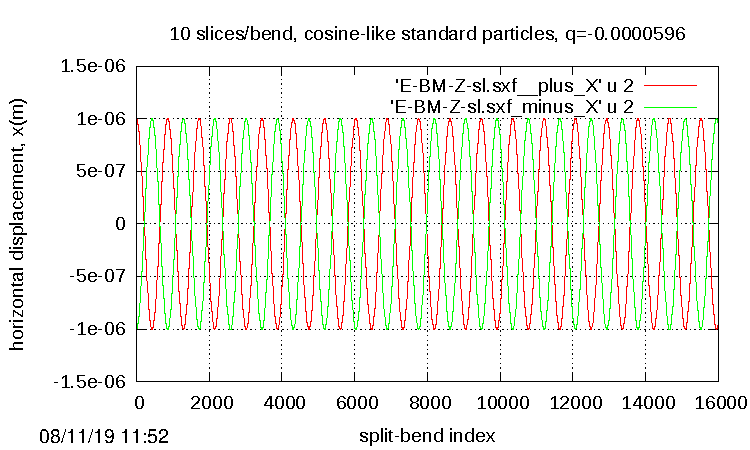
\includegraphics[scale=1.0]{pdf/Fig_I-3-sl-t.pdf} 
  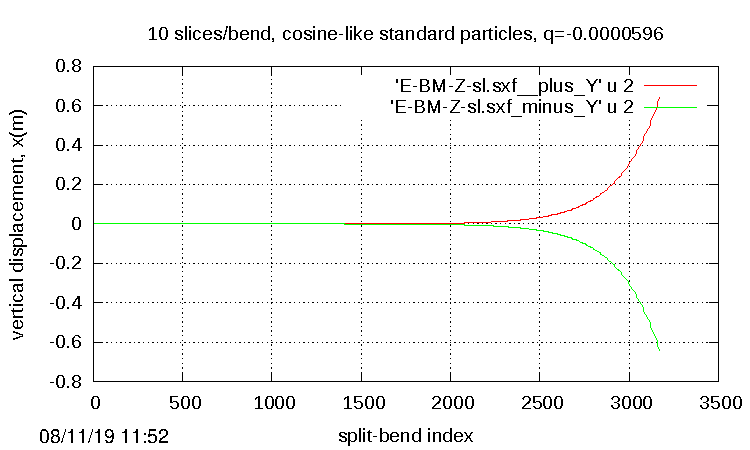
\includegraphics[scale=1.0]{pdf/Fig_I-3-sl-b.pdf} 
\caption{\label{fig:unchanged-q-value}
{\tt E\_BM\_Z-sl.sxf}: }
\end{figure}

\clearpage

\subsubsection{Ten SXF slices per bend, each with two TEAPOT slices, retuned $q$-value\label{sect:pre-sliced-modQ} }
To restore vertical stability the lumped quadrupole value has been adjusted from
$q=-0.0000596$ to $q=-0.002020$, which correspods to focal length $f=1/q\approx500$\,m,
and is quite weak for a six meter long cell length.
\begin{figure}[htbp] 
  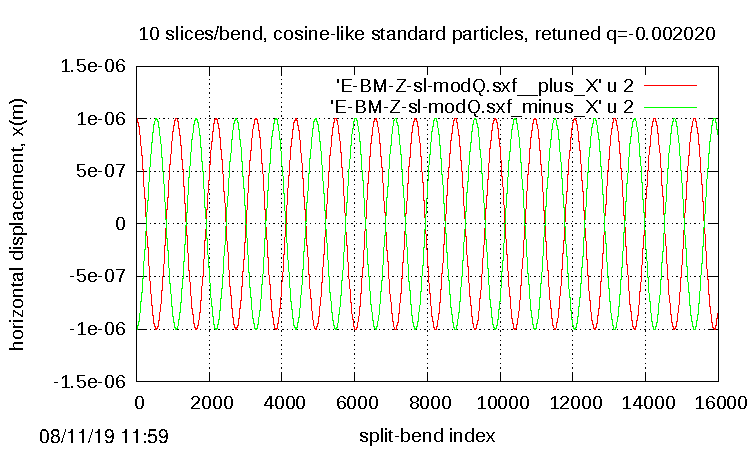
\includegraphics[scale=1.0]{pdf/Fig_I-3-sl-modQ-t.pdf} 
  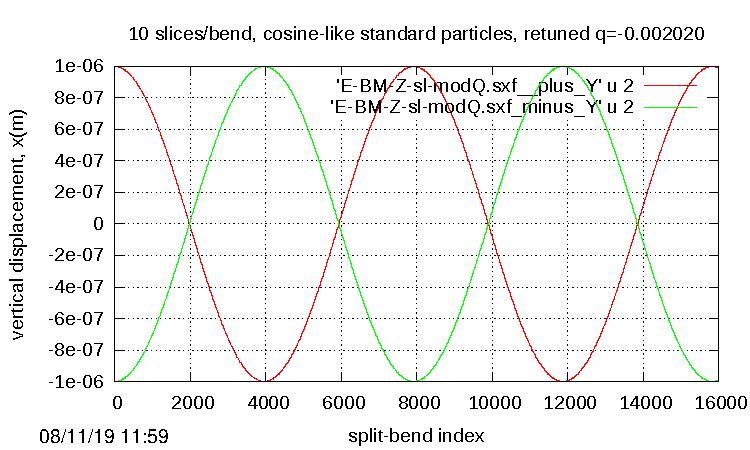
\includegraphics[scale=1.0]{pdf/Fig_I-3-sl-modQ-b.pdf} 
\caption{{\tt E\_BM\_Z-sl-modQ.sxf}: }
\end{figure}


\clearpage
\subsection{Lattice E\_BM\_M1.0, $m=-1$, bending results}
%
\begin{table}[h]
\caption{\label{tbl:benchmarkParams.M1.0}E\_TEAPOT comparisons for
{\tt ./tracker ./data/E\_BM\_M1.0.sxf 30 -1 > \& ! JTout}.
All {\tt typ} numerical differentiation displacements are proportional to {\tt tiny}.
} 
\medskip
\centering
\begin{tabular}{|c|c|c|c|c|c|c|c|c|}           \hline
file name         & variable name     & unit & linearized    & 2 slices/bend & $\Delta$'s  \\
                  &                   &      &   MAPLE       &     ETEAPOT   &             \\ \hline
cells/arc         & {\tt NCellPerArc} &      &      20       &               &             \\
bend radius       &  {\tt r0}         &  m   &     40.0      &               &    \\
half drift length &  {\tt Ldh}        &  m   &      1.0      &               &    \\
half bend per cell & {\tt Thetah}     &  r   &   0.078539816 &               &    \\
half bend length  & {\tt Leh}         &  m   &    3.141592   &               &    \\
circumference     & {\tt circum}      &  m   &   331.327     &               &    \\
inverse focal length &  {\tt q}       & 1/m  &    -0.002019  &               &    \\ 
field index       &  {\tt m}          &      &     -1.0      &               &    \\ \hline
 {\tt tiny=1.0e-6} &                  &      &               &               &     \\ \hline 
horizontal beta  & {\tt betax}        &  m   &    35.9237    &  35.8566      &  -0.0671 \\ 
vertical beta     & {\tt betay}       &  m   &   264.1820    & 251.8522      &  -12.3298 \\ 
horizontal tune  &  {\tt Qx}          &      &     1.4605    &   1.4620      &  0.0015 \\ 
vertical tune     &  {\tt Qy}         &      &     0.2002    &   0.2102      &  0.0100 \\ \hline
 {\tt tiny=1.0e-5} &                  &      &               &               &          \\ \hline 
horizontal beta  & {\tt betax}        &  m   &    35.9237    &  35.8566      &  -0.0671    \\ 
vertical beta     & {\tt betay}       &  m   &   264.1820    & 251.8522      & -12.3298   \\ 
horizontal tune  &  {\tt Qx}          &      &     1.4605    &   1.4620      &  0.0015 \\ 
vertical tune     &  {\tt Qy}         &      &     0.2002    &   0.2102      &  0.0100 \\ \hline
 {\tt tiny=1.0e-4} &                  &      &               &               &     \\ \hline 
horizontal beta  & {\tt betax}        &  m   &    35.9237    &  35.8582      & -0.0655 \\ 
vertical beta     & {\tt betay}       &  m   &   264.1820    & 251.8492      & -12.3328   \\ 
horizontal tune  &  {\tt Qx}          &      &     1.4605    &   1.4620      &  0.0015\\ 
vertical tune     &  {\tt Qy}         &      &     0.2002    &   0.2102      &  0.0100\\ \hline
 {\tt tiny=1.0e-3} &                  &      &               &               &     \\ \hline 
horizontal beta  & {\tt betax}        &  m   &    35.9237    &   36.0209     & 0.0972 \\ 
vertical beta     & {\tt betay}       &  m   &   264.1820    &  251.5553     & -12.6267 \\ 
horizontal tune  &  {\tt Qx}          &      &     1.4605    &    1.4621     &  0.0016 \\ 
vertical tune     &  {\tt Qy}         &      &     0.2002    &     0.2103    &  0.0101 \\ \hline
\end{tabular}
\end{table}
%

\begin{figure}[htbp] 
  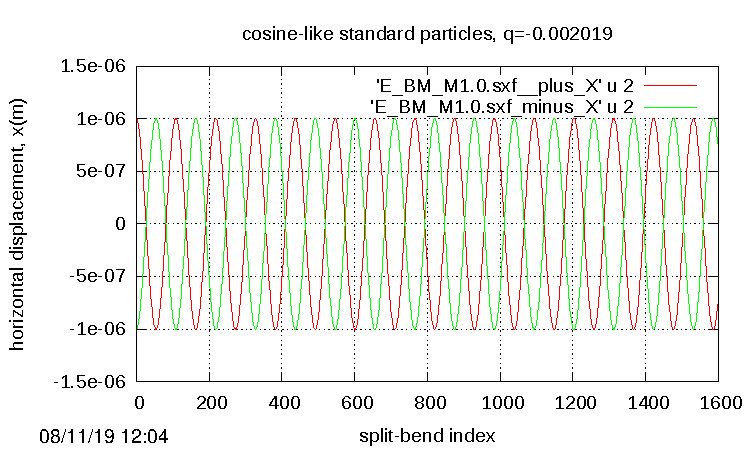
\includegraphics[scale=1.0]{pdf/Fig_I-4t.pdf} 
  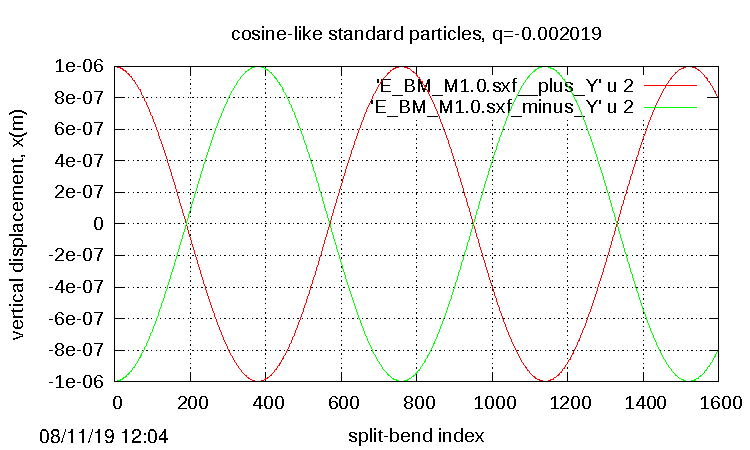
\includegraphics[scale=1.0]{pdf/Fig_I-4b.pdf} 
\caption{E\_BM\_M1.0.sxf: Horizontal Displacement: 10 turns, 1 sample per bend. 
$Q_x\approx$ 14.5 osc/10turns=1.45 osc/turn. 
The integer part of the tune is [$Q_x$] = 1. Vertical Displacement: 10 turns, 1 sample per bend. 
$Q_y\approx$ 2.1 osc/10turns=0.21 osc/turn. The integer part of the tune is [$Q_y$] = 0.}
\end{figure}


\clearpage

\subsection{Dependence on ETEAPOT Slicing Granularity}
The effect of finer ETEAPOT slicing is investigated in Tables~\ref{tbl:benchmarkParams.P1.0_},
\ref{tbl:benchmarkParams.Z_} and \ref{tbl:benchmarkParams.M1.0_}.  Doubling the slicing 
from 2 slices/bend to 4 slices/bend has little effect on the derived lattice parameters.
As in earlier parameter determinations, the vanishing differences for $m=1$ suggest that 
the main deviations are due more to perturbation away from $m=1$ than to overly-coarse slicing.
%
\begin{table}[h]
\caption{\label{tbl:benchmarkParams.P1.0_}E\_TEAPOT comparisons for
{\tt ./tracker ./data/E\_BM\_P1.0.sxf 30 1 > \& ! JTout}.  {\tt tiny=1.0e-6}.
} 
\medskip
\centering
\begin{tabular}{|c|c|c|c|c|c|c|c|c|c|c|}           \hline
file name         & variable name     & unit  &   linearized  & 2 sl./bend & $\Delta$'s & 4 sl./bend & $\Delta$'s  \\ \hline
cells/arc         & {\tt NCellPerArc} &       &        20     &  & & &        \\
bend radius       &  {\tt r0}         &  m    &       40.0    &  & & &        \\
half drift length &  {\tt Ldh}        &  m    &        1.0    &  & & &        \\
half bend per cell & {\tt Thetah}     &  r    &  0.078539816  &  &  & &       \\
half bend length  & {\tt Leh}         &  m    &   3.141592    &  &  & &       \\
circumference     & {\tt circum}      &  m    &    331.327    &  &  & &       \\ 
inverse focal length &  {\tt q}       & 1/m   &     0.0019075 &  & & &        \\
field index       &  {\tt m}          &       &         1.0   &  & & &         \\ \hline 
horizontal beta  & {\tt betax}       &  m     &   36.191030   &   36.19103 & & 36.19103 &        \\
vertical beta     & {\tt betay}       &  m    &  262.236988   &  262.23701 & & 262.23701 &        \\
horizontal tune  &  {\tt Qx}         &        &    1.458782   &    1.45878 & & 1.45878 &        \\ 
vertical tune     &  {\tt Qy}         &       &    0.200472   &    0.20047 & & 0.20047 &        \\ \hline
\end{tabular}
\end{table}
%

%
\begin{table}[h]
\caption{\label{tbl:benchmarkParams.Z_}E\_TEAPOT comparisons for
{\tt ./tracker ./data/E\_BM\_Z.sxf 30 0 > \& ! JTout}. {\tt tiny=1.0e-6}.
}
\medskip
\centering
\begin{tabular}{|c|c|c|c|c|c|c|c|c|c|c|}           \hline
file name         & variable name     & unit  &  linearized  & 2 sl./bend  & $\Delta$'s & 4 sl./bend & $\Delta$'s \\ \hline
cells/arc         & {\tt NCellPerArc} &       &       20     &   & & &     \\
bend radius       &  {\tt r0}         &  m    &      40.0    &   & & &   \\
half drift length &  {\tt Ldh}        &  m    &     1.0      &   & & &   \\
half bend per cell & {\tt Thetah}     &  r    &  0.078539816 &   & & &   \\
half bend length  & {\tt Leh}         &  m    &  3.141592    &   & & &   \\
circumference     & {\tt circum}      &  m    &   331.327    &   & & &   \\ 
inverse focal length &  {\tt q}       & 1/m   & -0.00005960  &   & & &   \\
field index       &  {\tt m}          &       &  1.0e-10     &   & & &   \\ \hline
horizontal beta  & {\tt betax}       &  m     &  36.101819   &   36.07949 & & 36.09624  &  \\ 
vertical beta     & {\tt betay}       &  m    & 263.620065   &  261.46880 & & 263.07673 &  \\
horizontal tune  &  {\tt Qx}         &        &   1.457801   &    1.45813 & & 1.45788  &  \\
vertical tune     &  {\tt Qy}         &       &   0.200044   &    0.20177 & & 0.20048  &  \\ \hline        
\end{tabular}
\end{table}
%

%
\begin{table}[h]
\caption{\label{tbl:benchmarkParams.M1.0_}E\_TEAPOT comparisons for
{\tt ./tracker ./data/E\_BM\_M1.0.sxf 30 -1 > \& ! JTout}. {\tt tiny=1.0e-6}.
} 
\medskip
\centering
\begin{tabular}{|c|c|c|c|c|c|c|c|c|c|}           \hline
file name         & variable name     & unit & linearized    & 2 sl./bend & $\Delta$'s &4 sl./bend & $\Delta$'s   \\ \hline
cells/arc         & {\tt NCellPerArc} &      &      20       &  &  & &  \\
bend radius       &  {\tt r0}         &  m   &     40.0      &  &  & & \\
half drift length &  {\tt Ldh}        &  m   &      1.0      &  &  & & \\
half bend per cell & {\tt Thetah}     &  r   &   0.078539816 &  &  & & \\
half bend length  & {\tt Leh}         &  m   &    3.141592   &  &  & & \\
circumference     & {\tt circum}      &  m   &   331.327     &  &  & & \\
inverse focal length &  {\tt q}       & 1/m  &    -0.002019  &  &  & & \\ 
field index       &  {\tt m}          &      &     -1.0     &  &  & & \\ \hline
horizontal beta  & {\tt betax}       &  m   &    35.923719   &  35.85659 & & 35.90695 & \\ 
vertical beta     & {\tt betay}       &  m   &  264.182337   & 251.85222 & & 260.92409 & \\ 
horizontal tune  &  {\tt Qx}         &      &     1.460454   &   1.46204 & &   1.46085 & \\ 
vertical tune     &  {\tt Qy}         &      &    0.200242   &   0.21021 & &  0.20278 & \\ \hline
\end{tabular}
\end{table}
%




\clearpage

\section{Comments and Conclusions}
For the $m=1$ case, there is nearly exact agreement between the linearized analytic formulae and the tracking formalism. 
This is ``as should be'', but far from automatic. The equations of the linearized transfer matrix formalism and the 
arbitrary-amplitude Munoz-Pavic seem utterly different. So the close agreement confirms \emph{both} approaches.
This comment mainly applies to the ``in-plane'' horizontal motion. Agreement of the ``out-of-plane'' vertical
motion, where the overall agreement is less impressive, especially as investigated with a pre-sliced SXF lattice,
in Sections~\ref{sect:pre-sliced} and \ref{sect:pre-sliced-modQ}. Vertical steering errors, however small, are 
amplified by the weak vertical focusing of the lattice. 

The agreement for $m\ne1$ is excellent, but clearly not as good as for $m=1$. This strongly suggests that the 
(artificial) perturbative kick compensation is not quite perfect. It is also not surprising that the deviation 
is proportional to $(m-1)^2$; and that, for $m=1$, the kick correction strength vanishes.

For most practical purposes, the code performance in the parameter range $-1\le m\le 1$ has been shown to 
be satisfactory. 
\clearpage





\begin{thebibliography}{99}
\bibitem{pEDM}
Storage Ring EDM Collaboration, \emph{A Proposal to Measure the
Proton Electric Dipole Moment with $10^{-29}\,$e-cm Sensitivity,}
especially Appendix 1. October, 2011

\bibitem{Moller}
C. M\o ller, \emph{The Theory of Relativity,} Clarendon Press,
Oxford, 1952, 

\bibitem{Munoz}
G. Mu\~{n}oz and I. Pavic, \emph{A Hamilton-like vector for
the special-relativistic Coulomb problem,} 
Eur. J. Phys. {\bf 27}, 1007-1018, 2006

\bibitem{Talman}
R. Talman, \emph{Geometric Mechanics,} John Wiley and Sons, 2000

\bibitem{Aguirregabiria}
J. Aguirregabiria et al., 
Archiv:physics/0407049v1 [physics.ed-ph] 2004, 

\bibitem{Torkelsson}
U. Torkelsson, Eur. J. Phys., {\bf 19}, 459, 1998, 

\bibitem{Boyer}
T. Boyer, Am. J. Phys. {\bf 72} (8) 992, 2004

\end{thebibliography}


\end{document}

